\chapter{Sex Hormone System}
\label{ch:sex-hormones}

Why do females respond better to some cancer treatments while males benefit more from others? This chapter reveals how sex hormones orchestrate immune responses --- and shows how estrogen at moderate levels actually boosts the immune system, explaining the female advantage in cancer survival.

This chapter describes the sex hormone subsystem, which models the immunomodulatory effects of estrogen, testosterone, and progesterone on the tumor microenvironment. Sex-specific differences in hormone profiles produce distinct immune dynamics, contributing to the well-documented sex disparity in RCC incidence and treatment response.

%% ====================================================================
\section{Biological Basis}
\label{sec:hormone-bio}

Renal cell carcinoma exhibits a pronounced sex disparity with males affected approximately twice as often as females, yet treatment efficacy varies significantly between sexes. Estrogen exerts complex, concentration-dependent effects: at low to moderate levels, it promotes Th1-type immune responses, enhances IFN-$\gamma$ production, and stimulates T cell activation; at high concentrations, it shifts towards Th2-type responses and increases inhibitory checkpoint engagement. Testosterone is generally immunosuppressive at elevated levels, reducing Th1 proliferation, decreasing IFN-$\gamma$ production, and promoting immune checkpoint engagement. Progesterone has minimal effects at low levels, mildly enhances checkpoint inhibition at moderate levels, and strongly suppresses Th1 proliferation while promoting Th2 differentiation at high concentrations. These clinical observations suggest that sex hormones modulate the immune response in ways that affect both tumor susceptibility and treatment efficacy.

%% ====================================================================
\section{Hormone Agent Model}
\label{sec:hormone-agent}

Sex hormones are modeled as discrete agents (estrogen, testosterone, progesterone) that diffuse through the simulation grid, interact with nearby immune cells, and decay over time. The \texttt{SexHormone} class inherits from \texttt{repast4py.core.Agent} and is registered as agent type ID 16. Hormones are spawned from blood vessel positions with sex-specific probabilities (male: estrogen 0.2, progesterone 0.1, testosterone 1.0; female: estrogen 0.9, progesterone 0.8, testosterone 0.2). Once spawned, hormones perform biased random walk through the grid with drift away from blood vessels, and those exiting grid boundaries are removed, providing natural hormone clearance with effective lifespan of approximately 50 steps.

\begin{table}[H]
\centering
\caption{Hormone spawn probabilities by patient sex.}
\label{tab:hormone-spawn}
\begin{tabular}{lccc}
\toprule
\textbf{Sex} & \textbf{Estrogen} & \textbf{Progesterone} & \textbf{Testosterone} \\
\midrule
Male   & 0.2 & 0.1 & 1.0 \\
Female & 0.9 & 0.8 & 0.2 \\
\bottomrule
\end{tabular}
\end{table}

%% ====================================================================
\section{Hormone Effects on T Cells}
\label{sec:hormone-effects}

T cells detect sex hormones via \texttt{perceive\_sex\_hormone()} method, maintaining dictionaries of perceived hormone levels that decay by 10\% per step. The \texttt{CellHormonalInfluenceEffect} enumeration defines 17 effect channels through which hormones modulate T cell behavior:

\begin{longtable}{lp{9cm}}
\caption{Hormonal influence effect channels.}
\label{tab:hormonal-effects} \\
\toprule
\textbf{Effect} & \textbf{Description} \\
\midrule
\endfirsthead
\toprule
\textbf{Effect} & \textbf{Description} \\
\midrule
\endhead
\bottomrule
\endlastfoot
KILL\_RATE            & Cytotoxic kill rate modulation. \\
PROLIFERATION         & General proliferation rate. \\
APOPTOSIS             & Programmed cell death susceptibility. \\
ACTIVATION            & T cell activation state. \\
DIFFERENTIATION       & Differentiation probability (e.g., naive to effector). \\
TH1\_PROLIFERATION    & Th1-specific proliferation. \\
TH2\_PROLIFERATION    & Th2-specific proliferation. \\
IL\_4                 & Interleukin-4 signaling effect. \\
IL\_6                 & Interleukin-6 signaling effect. \\
IL\_13                & Interleukin-13 signaling effect. \\
IFN\_GAMMA            & Interferon-gamma signaling effect. \\
TNF\_ALPHA            & Tumor necrosis factor alpha effect. \\
MHC\_I\_UPREGULATION  & MHC class I expression modulation. \\
MHC\_II\_UPREGULATION & MHC class II expression modulation. \\
COSTIMULATION\_CD28   & CD28 costimulatory signal strength. \\
CTLA4\_SUPPRESSION    & CTLA-4 inhibitory checkpoint engagement. \\
PD1\_INHIBITION       & PD-1 inhibitory checkpoint engagement. \\
\end{longtable}

Perceived hormone levels are normalized to [0,1] scale and mapped to concentration regimes (low $<0.33$, medium $0.33$-$0.66$, high $\geq 0.66$). Effects are weighted by hormone-specific importance: $w_{\text{estrogen}} = 0.45$, $w_{\text{testosterone}} = 0.30$, $w_{\text{progesterone}} = 0.25$.

%% ====================================================================
\section{Sex Drift}
\label{sec:sex-drift}

The model implements population-level sex drift that adjusts CD8+ naive T cell populations based on patient sex, reflecting testosterone's stimulation of CD8+ T cell production in the thymus. The drift operates as gradual population adjustment over 15 steps with maximum drift $d_{\max} = 0.25$: $\delta = d_{\max}/n$ per step, where direction $\sigma = +1$ for males (population increase) and $\sigma = -1$ for females (population decrease). Step factor $f_{\text{step}} = 1 + \sigma \cdot \delta$ determines duplication probability (males) or removal probability (females), producing approximately ±25% population change over 15 steps.

\begin{equation}
\label{eq:drift-per-step}
\delta = \frac{d_{\max}}{n}, \qquad f_{\text{step}} = 1 + \sigma \cdot \delta
\end{equation}

\begin{figure}[htbp]
\centering
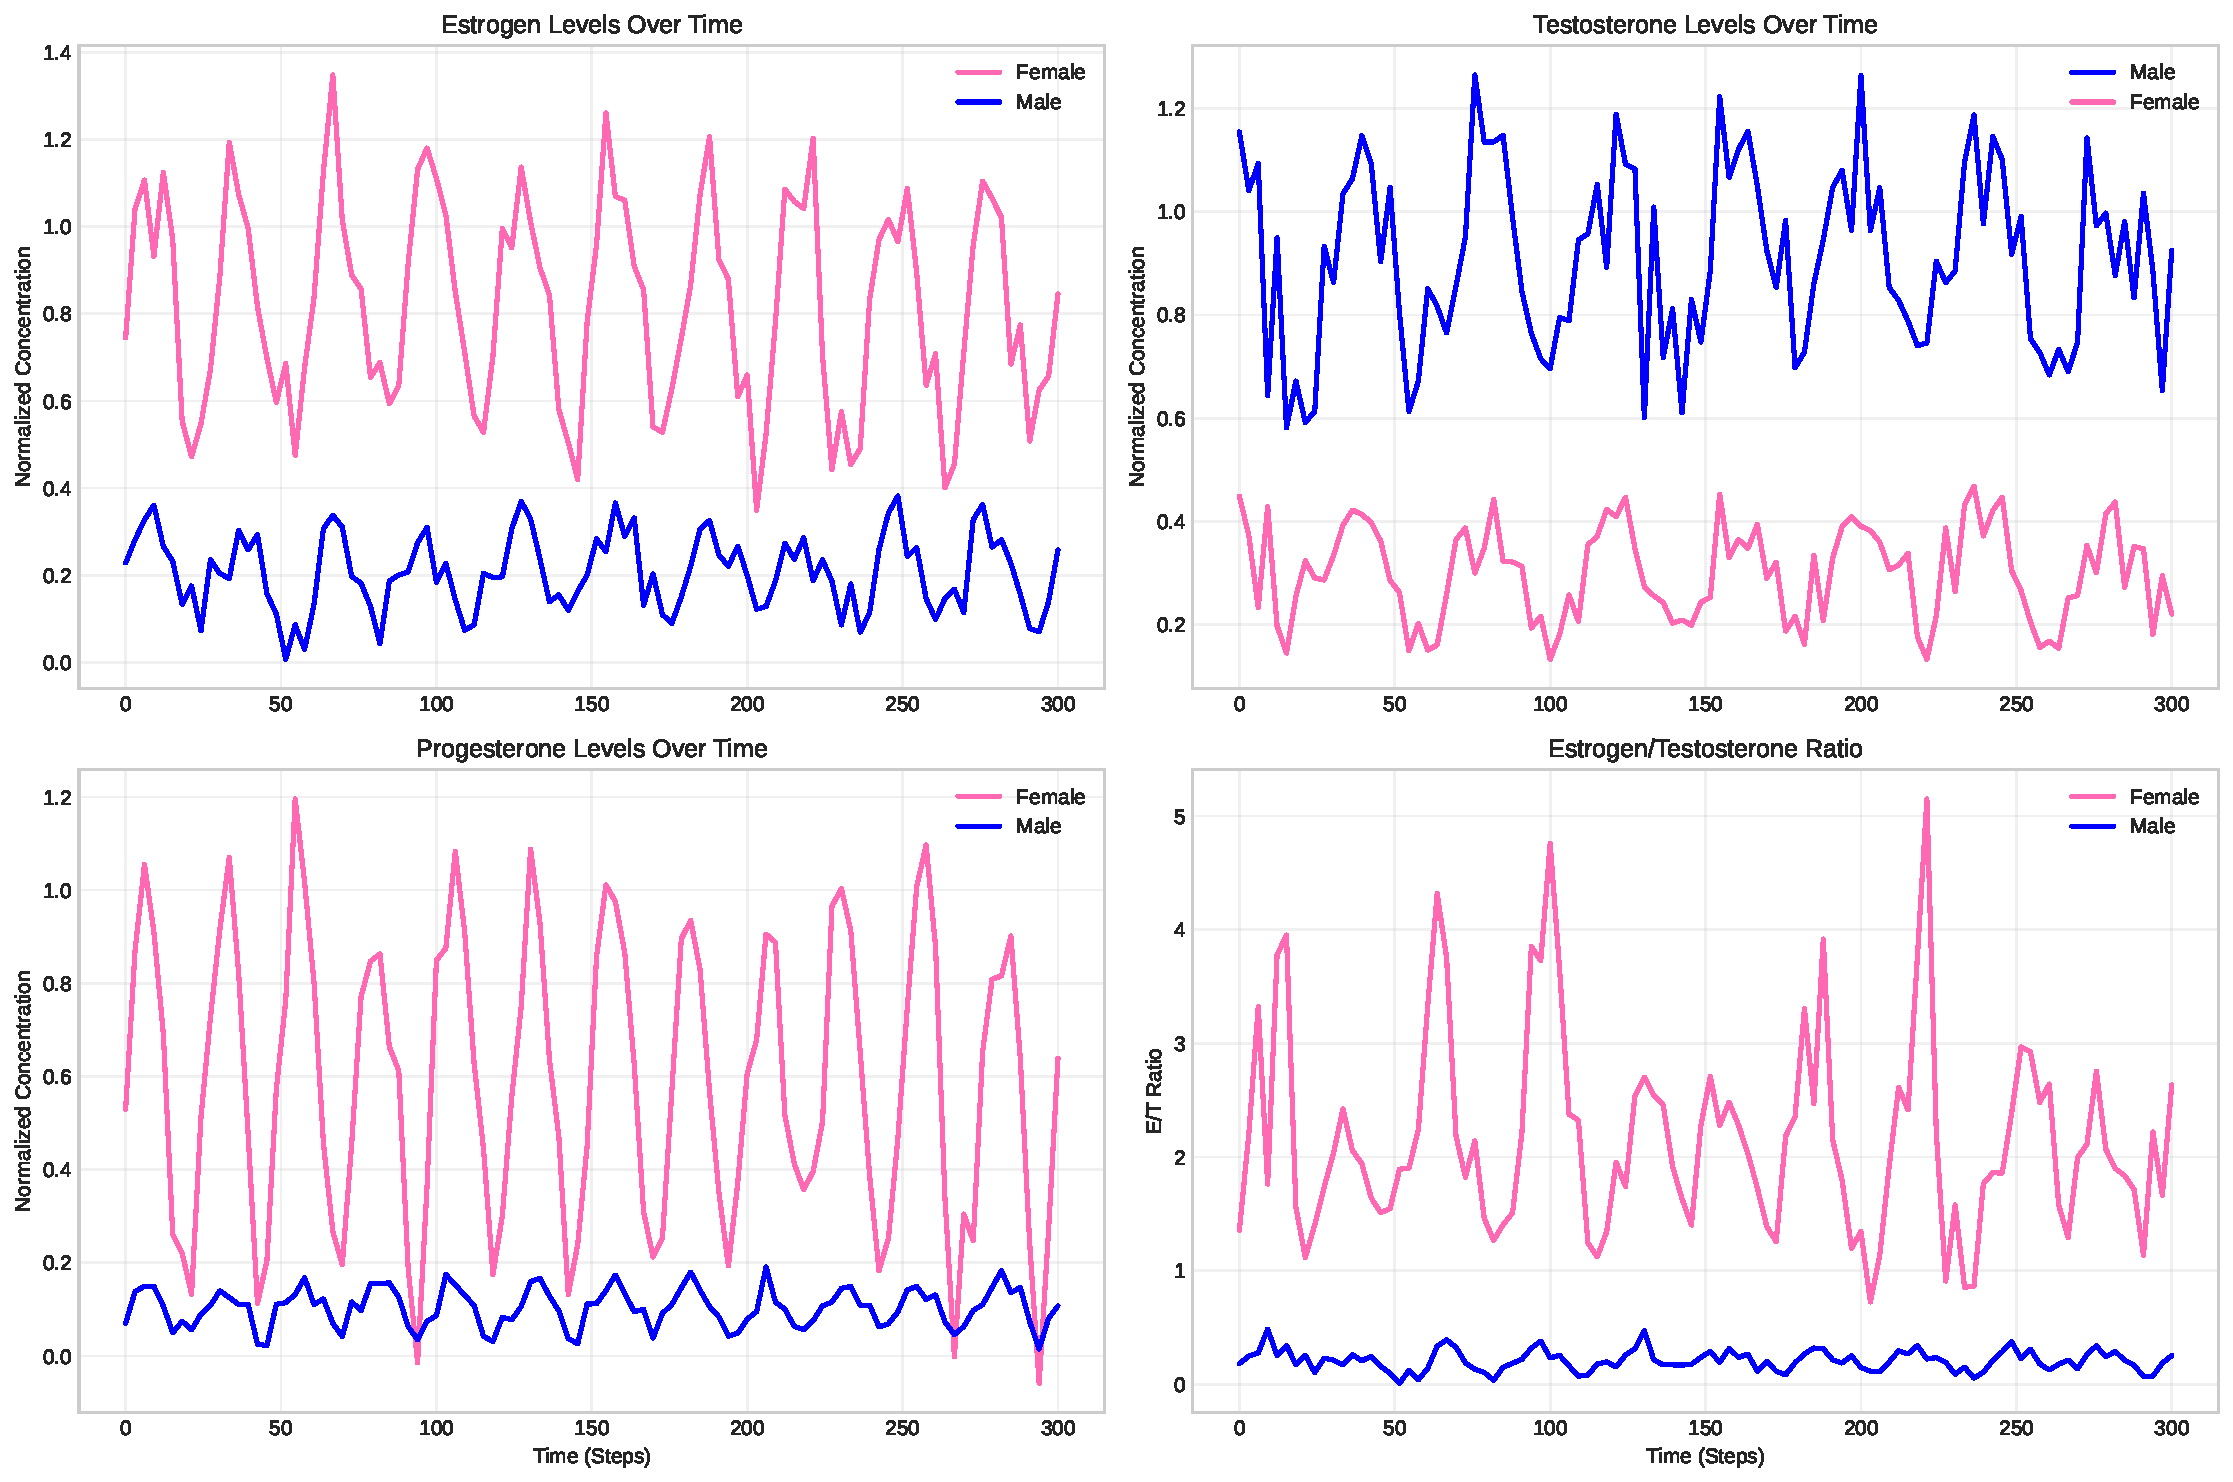
\includegraphics[width=0.85\textwidth]{figures/hormone_dynamics.pdf}
\caption{Sex hormone dynamics over time showing the evolution of estrogen, testosterone, and progesterone levels in the tumor microenvironment. The hormone concentrations fluctuate based on sex-specific spawning rates, cellular consumption, and spatial diffusion patterns.}
\label{fig:hormone_dynamics}
\end{figure}